\documentclass[12pt]{article}

\usepackage[T1]{fontenc}
\usepackage[utf8]{inputenc}
\usepackage[english]{babel}
\usepackage{booktabs}
\usepackage{multirow}
\usepackage{graphicx}
\usepackage[table,xcdraw]{xcolor}
\usepackage{longtable}
\usepackage{indentfirst}
\usepackage[margin=2.5cm]{geometry}
\usepackage[hidelinks]{hyperref}
\usepackage{graphicx}
\usepackage{amsmath}




\graphicspath{ {./images/} }

\renewcommand{\baselinestretch}{1.5} % spacing

\usepackage[backend=bibtex, sorting=none]{biblatex}
\bibliography{bibl}

\title{Artificial Intelligence Report - The 15-puzzle}
\author{Aneta Andrzejewska 200285 \and Michał Kącki 203206}
\date{20 November 2018}


\begin{document}

\pagenumbering{gobble}

\maketitle
\newpage

\tableofcontents
\newpage

\pagenumbering{arabic}
\setcounter{page}{3}

\section{Introduction}
\subsection{Background}

The 15-puzzle game is a sliding puzzle consisting of a frame of numbered square tiles in random order with one tile missing \cite{15-puzzle}. The goal of the game is to shift the tiles in such a way that they are in order using the empty space. The game comes in different settings characterised by the number of slides. The two most popular sizes are $3\times3$ and $4\times4$, which are called the 8- and 15-puzzle, respectively.

The n-puzzle game is a popular problem in computer science used to model different algorithms using various heuristics as a means to solve the puzzle. This is possible because all the states, i.e. placings of the slides, which a board for the puzzle can be in, could be represented as nodes of a graph, where every node has three or four children, representing the state of the board after moving the empty space in every direction. Three children are considered when the empty space is located on the border of the board.

\subsection{Goal}

The goal of the laboratory was to implement the 15-puzzle game alongside a few algorithms used for solving it and analyse them in terms of their performance. The considered algorithms were:

\begin{itemize}
    \item Breadth-first search (BFS)
    \item Depth-first search (DFS)
    \item Iterative deepening depth-first search (IDDFS)
    \item Best-first search (BFS)
    \item A*
    \item Simplified Memory Bounded A* (SMA*)
\end{itemize}

In addition to the above requirements, the program should also provide the user with a possibility to choose one of two heuristics for best-first search, A* and SMA*. It should be possible to start the program and pass relevant arguments via the command line. The last requirement was that the program should be able to print the sequence of moves of the empty space leading to obtaining the solved puzzle.

\subsection{Description of the algorithms}

\subsubsection{Breadth-first search (BFS)}

Breadth-first search is the simplest method of traversing a graph. The idea is that each vertex at the present depth needs to be expanded before descending further down the tree. While definitely simple, BFS slows down immensely when the considered graph is too large.

\begin{figure}[h]
    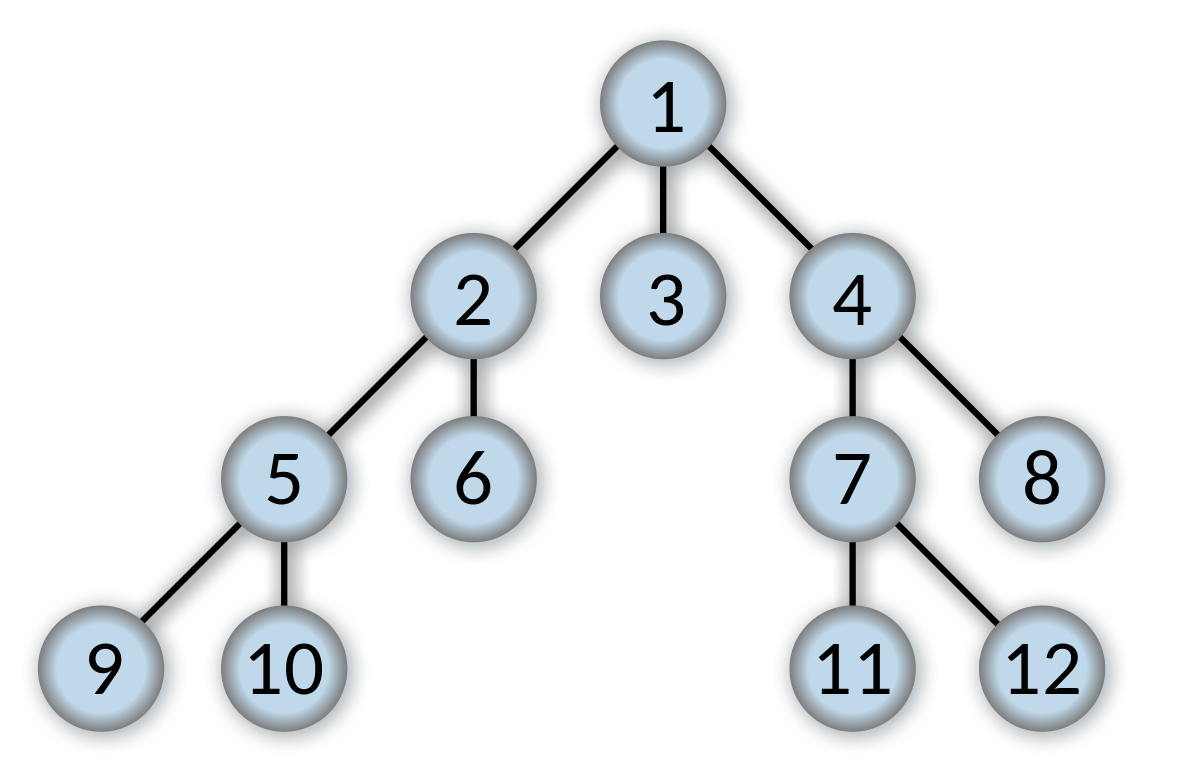
\includegraphics[width=0.75\textwidth]{bfs}
    \centering
    \caption{Breadth-first search traversal order \cite{bfs_image}}
\end{figure}

\subsubsection{Depth-first search (DFS)}

Depth-first search is another simple method of traversing graphs. It differs from the BFS in that it prioritises expanding one path towards the bottom of the graph instead of visiting each vertex at a particular depth first. When a path is completely expanded, the algorithm goes back to expand the omitted nodes.

\begin{figure}[h]
    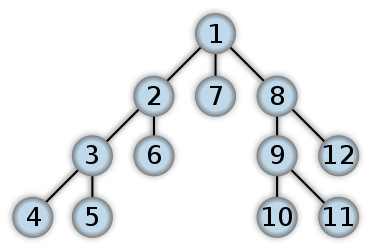
\includegraphics[width=0.75\textwidth]{dfs}
    \centering
    \caption{Depth-first search traversal order \cite{dfs_image}}
\end{figure}

\subsubsection{Iterative deepening depth-first search (IDDFS)}

Iterative deepening depth-first search algorithm is basically the improved version of DFS in that it also utilises the strategy present in BFS. IDDFS uses a parameter called ``depth limit'', which tells the algorithm how deep to traverse down the tree before running BFS on a particular level. IDDFS may be thought of as a combination of DFS and BFS - it takes space-efficiency from the former and completeness from the latter effectively performing a lot better than the aforementioned algorithms.

\begin{figure}[h]
    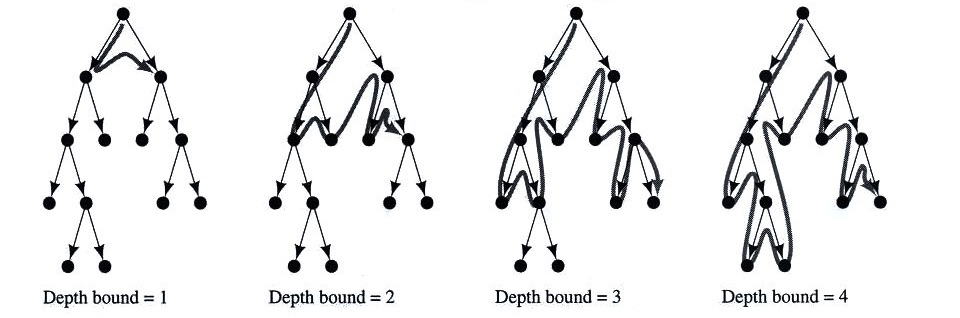
\includegraphics[width=0.75\textwidth]{iddfs}
    \centering
    \caption{Iterative deepening depth-first search traversal order \cite{iddfs_image}}
\end{figure}

\subsubsection{Best-first search (BFS)}

Best-first search is quite different from all the above methods. To arrive at a solution it uses a heuristic evaluation function telling the algorithm which vertex should now be expanded. There exists a plethora of different heuristics to choose from. One of the most popular is called a ``pure heuristic''. When utilising that heuristic, the algorithm tries to assess how close a particular path is to a solution and first chooses those that are the closest. When using heuristics, each vertex has a weight associated with it.

\begin{figure}[h]
    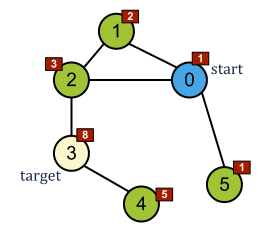
\includegraphics[scale=0.75]{bfs2}
    \centering
    \caption{Best-first search traversal order showing the weights of the nodes \cite{bfs2_image}}
\end{figure}

\subsubsection{A*}

A* algorithm is a kind of best-first search as it uses heuristics as well. However, instead of considering only a path from the current node to a solution, the whole cost of arriving at the currently considered vertex is also taken into consideration. A* strategy is described by the following equation:

\[
f(n) = g(n) + h(n),
\]
where $n$ indicates the next vertex on the path, $g(n)$ is the cost from the root vertex to $n$ and $h(n)$ is the aforementioned heuristic function evaluating the cost of the cheapest path from the vertex $n$ to the solution.

\begin{figure}[h]
    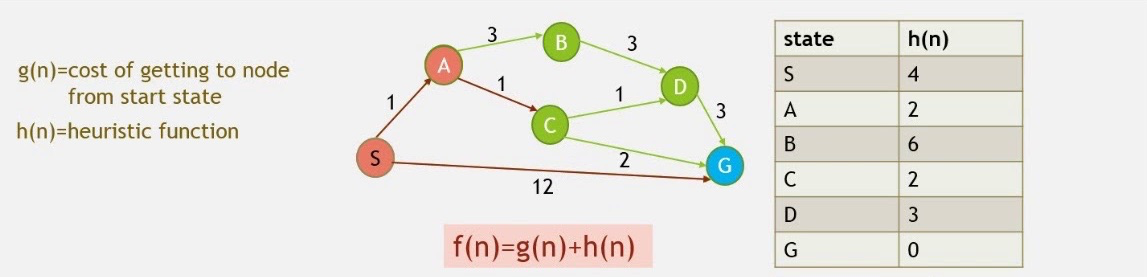
\includegraphics[width=\textwidth]{astar}
    \centering
    \caption{A* traversal order \cite{astar_image}}
\end{figure}

\subsubsection{Simplified Memory Bounded A* (SMA*)}

Simplified Memory Bounded A* is the successor of MA* which takes the concept of A* and applies memory bounds on the container storing vertices yet to be visited. When the container is full, the most costly nodes (those with the highest f-cost) are dropped to make a place for the nodes that might be a better choice. To prevent infinite looping the f-cost values are backed up through the tree. When it is needed, some nodes are re-expanded. SMA* simplifies the logic of MA* and in fact, performs better than its overcomplicated predecessor. First of all, it uses a binary tree to store the list of vertices that need to be expanded, which is a more efficient data structure than the one originally used in MA*. Also, the backup procedure is started only when a vertex has been fully expanded, which speeds up the execution time of the algorithm \cite{GCAI2017:Enhanced_Simplified_Memory_bounded_Star}.

\begin{figure}[h]
    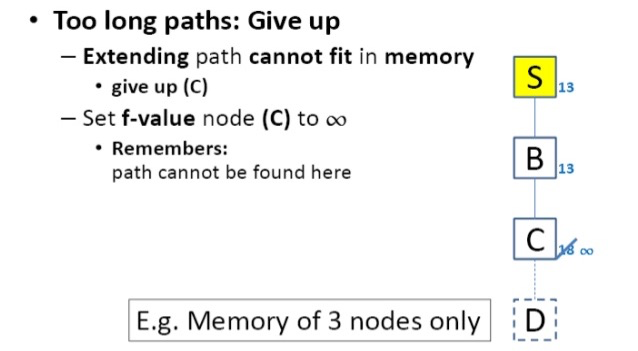
\includegraphics[width=0.75\textwidth]{smastar}
    \centering
    \caption{SMA* logic \cite{smastar_image}}
\end{figure}

\section{Implementation}

\subsection{Language}

The project was written in Eclipse IDE using Java programming language with JDK 8. It was created with use of Apache Maven to handle dependencies between sub-projects and external libraries. 

\subsection{Functional requirements}
\subsubsection{Command line arguments}

The first program can be started from the command line and it takes the following parameters:

\begin{itemize}
    \item -b / --bfs order (BFS)
    \item -d / --dfs order (DFS)
    \item -i / --idfs order (IDDFS)
    \item -h / --bf id-of-heuristics (best-first search)
    \item -a / --astar id-of-heuristics (A*)
    \item -s / --sma id-of-heuristics (SMA*)
    \item --help (printing help)
\end{itemize}

\subsubsection{Order and heuristics}

BFS, DFS and IDDFS require the order in which successors of given state are processed to be passed. ``R'' indicates that the nodes can be chosen randomly, whereas a string ``R L U D'' means the following search order: right, left, up, down.

Best-first search, A* and SMA* require an ID of a heuristic to be passed. The implemented ones are:

\begin{itemize}
    \item 0 / --zero (zero heuristics)
    \item  1 / --inpos (incorrect position heuristics)
    \item 2 / --mand (Manhattan distance heuristics)
\end{itemize}

Zero heuristics means that every node answers with a value of 0, which implies that every node is considered as good as the others.

Incorrect position heuristics calculates how many tiles are in the wrong position - the less the value of the function, the better the tile configuration is.

Manhattan distance heuristics answers with the sum of distances from each tile's position to its correct place applying the Manhattan distance formula:

\[
    d(p, q) = |p_1 - q_1| + |p_2 - q_2|,
\]

where $d$ is the distance, $p$ and $q$ are the considered vectors and $(p_1, p_2)$, $(q_1, q_2)$ are their components.

\subsubsection{Input}

In the first line of standard input two integer values, R C are given: row count and column count, respectively, defining frame size. Subsequent R lines of standard input contain C space separated integer values describing a piece in the puzzle. Value 0 denotes the empty space in the given frame.

\subsubsection{Output}

When the first program finishes its work, it displays four lines of text. In the first line, a size of the puzzle is shown (rows $\times$ columns). The second line contains the initial order of tiles in the board. The third line contains the length of the sequence of moves leading to a correct solution, whereas the fourth line is filled with the aforementioned sequence of moves.

\subsubsection{Viewer}

Additionally, the second small program has been created, namely a ``viewer''. The viewer allows users to see what moves were performed to arrive at a solved board. It takes as an input an output of the first program and displays subsequent tiles configurations one step per second.

\subsection {Algorithm details}

\subsubsection{Breadth-first search (BFS)}

In the project BFS was implemented with use of a Queue collection that order elements in a FIFO (first-in-first-out) manner. Before the first iteration of the algorithm a root node of a graph is added to the queue. Then, for each element of the queue, a function checks whether the tile configuration is correct. If not, for a current element, children configurations are generated according to the given order of movement directions and added to the queue. Furthermore, an Set was created to hold history of generated tiles configurations in order to prevent a situation in which the same tile configuration will be added to the queue and checked for correctness multiple times. Tile configurations are added to the history set just after their generation.

\subsubsection{Depth-first search (DFS)}

Depth-first search algorithm was implemented with a Stack class that represents a last-in-first-out (LIFO) strategy. As in BFS a root node is first added to the stack, then in each iteration a check for correctness is made. In DFS before generation of new tile configuration a condition of maximal depth of a branch is checked. If a given branch satisfies this condition child configurations are generated. Then if a given child configuration was not checked before (is not in a history set) and is not already present in the stack, it is added to it. This time, tile configuration is added to the history set only after is was popped from the stack, and not immediately after generation.  

\subsubsection{Iterative deepening depth-first search (IDDFS)}

IDDFS was implemented similarly to the DFS algorithm. Roughly speaking it calls the same actions as DFS but in an iterative manner. In each iteration an algorithm goes to the certain depth starting from 1, which is then incremented if correct solution was not found. A new stack and a history set is created for each iteration. Then all steps are analogous to the DFS algorithm. The procedure is continued until a correct configuration is found or a condition of a maximal depth is reached.

 \subsubsection{Best-first search (BFS)}

Best-first search algorithm is the first algorithm that uses heuristics to find the correct configuration. From implementation perspective it is largely similar to Breadth-first search algorithm, however, instead of using FIFO queue, a priority queue is used. Priority of an element is calculated based on heuristics used.

\subsubsection{A*}

A* algorithm is in fact implemented as Best-first search algorithm but with different method of priority calculation. In A* not only the cost value g(n) is used but also a distance from the root is taken into account. Everything else is just like in Best-First search algorithm.


\subsubsection{Simplified Memory Bounded A* (SMA*)}

SMA* is the most complicated algorithm from all described ones. First of all it used two types of priority queues. Priority is defined exactly as in A* algorithm, however, it gets updated throughout the algorithm progress. First queue named open is ordered with this priority and it holds all of the elements that are to be processed. Second queue is named closed, and it is ordered with a reversed way, meaning elements with lowest priority will be served first. This queue is used to find which elements should be forgotten when a memory limit is reached. Next two structures used are aimed to hold successors of a given board. They were implemented with use of a Map collections in which a tile configuration is a key and a list of possible children tile configurations are values. First map named availableSuccessorsMap holds all possible children configurations, which are those that can be generated from a given tile configuration excluding such configurations that were decided to be removed from memory. Next map, which is successorMap hold information about children configurations that are yet to be processed - if some branch would turn out to be unpromising algorithm gets a next child to process from the sucessorMap. Furthermore, a variable to hold current memory consumption is needed (named currentDepth). 

As usual, the algorithm starts by putting the root node into the open queue, also currentDepth is incremented. Then until the open queue is empty a tile configuration with highest priority is popped from it and returned if correct. If not, a process of a successor generation takes place. Initially a check is made whether sucessorMap contains the current tile configuration. If so, the successor is simply the next element from a children list taken from sucessorMap. The successor is then removed from this list, so that the algorithm will later know that this child has already been processed. If the sucessorMap does not contain the current tile configuration it means that none of its children were processed. Then the successor is taken as the first child from the list of possible children configuration taken from availableSuccessorsMap. 
The next part of the algorithm checks whether the successor was found. If so, an algorithms tests whether its configuration is correct and returns it if it is. If not, the procedure of defining value f(s) for the successor takes place. If the number of steps required to reach this configuration exceeds the memory limit f(s) is set to infinity - as this element should be marked as the first to be forgotten. If not f(n) is defined as:
\[
f(s) = max(f(n), g(s) + h(s).
\]
Then, such a successor is added to both queues, open and closed. 
On the other hand, if no successor was found, meaning all available children were processed, a backup procedure takes place. With this procedure costs are propagated through the graph and as a result priorities in nodes are recalculated so that most promising branches are first taken into account. It sets the f(n) value to be the lowest f(s) from all of the available children. Backup procedure is called recursively for parent node of a current node until root node is reached. After whole procedure is finished, current node is removed from both queues and currentDepth is incremented. 
Next part of the algorithm is called when memory limit is reached and it is aimed to forget the least promising node in order to make space for others. The node is chosen by polling from the closed queue. It is also removed from an open queue. Then the availableSuccessorsMap is updated so that it no longer includes the forgotten node. Then a parent node is added to both queues. If the parent node has no successors to be processed its f(n) is set to infinity, so that it will be first to be forgotten. The last step is decrementing of the currentDepth variable.  

In this way SMA* was implemented and it finds a solution withing a given memory limit. 

\section{Algorithms' analysis}

For every method of puzzle solving unit tests were created that were aimed to check if a method is able to solve given test cases and in what time.

\subsection {Test cases}

When it comes to test cases, two types of puzzles were analyzed - 8 puzzle and 15 puzzle, both with different difficulty level. Tile configurations that were used as test cases are presented in figure~\ref{puzzle-test}.

\begin{figure}[h]
    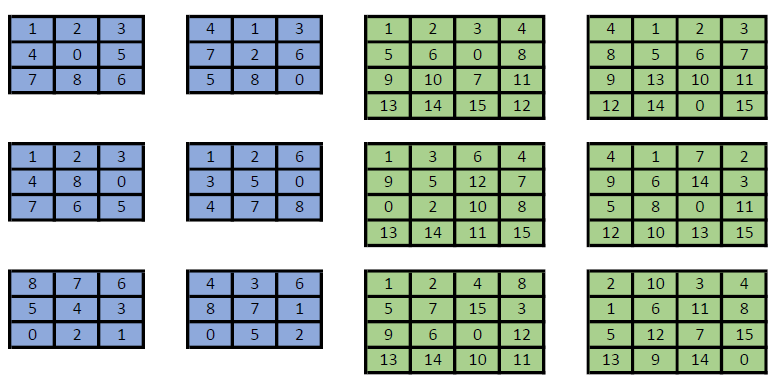
\includegraphics[width=\textwidth]{puzzle_test}
    \centering
    \caption{8 and 15 puzzle test cases}
    \label {puzzle-test}
\end{figure}

Each test case is presented in a form of a tile grid. Blue grids represent 8-puzzle problems, while green ones - 15 puzzle problem. Each of those grids contains NxN elements, where N is either 3 or 4 for 8-puzzle and 15-puzzle respectively. Tile 0 acts as an empty tile which will be able to preform movements. 

Each test case was fetched to JUnit tests of all algorithms. Then, for each of those test cases time of execution, length of the solution found, and a number of needed iterations was measured. All algorithms were tested with maximal depth of 100 and order of children generation:  RIGHT, DOWN, LEFT, UP. Results of those tests forms a bases for further algorithm comparison.

\subsection {Experiment results }

\subsubsection {8-puzzle}

In each of the test cases, both for 8-puzzle and 15-puzzle time of execution, number of needed iterations, and the length of the found solution was measured. Results for 8-puzzle are presented in the table~\ref{eight-puzzle-table}. I.P. and M.D. means Incorrect Position and Manhattan Distance Heuristics respectively. In the table results for test 0 heuristics is not shown, as it was not able to properly solve puzzles either due to its poor performance. In most cases Java Heap Space Exception was thrown for this heuristics.  


\begin{longtable}[h]{|
>{\columncolor[HTML]{C0C0C0}}c ccccccccc|}
\caption{8-puzzle test results}
\label{eight-puzzle-table}\\
\hline
Method & \cellcolor[HTML]{C0C0C0} & \cellcolor[HTML]{C0C0C0} & \cellcolor[HTML]{C0C0C0} & \multicolumn{2}{c}{\cellcolor[HTML]{C0C0C0}BestFS} & \multicolumn{2}{c}{\cellcolor[HTML]{C0C0C0}A*} & \multicolumn{2}{c|}{\cellcolor[HTML]{C0C0C0}SMA*} \\
Heuristics & \multirow{-2}{*}{\cellcolor[HTML]{C0C0C0}BFS} & \multirow{-2}{*}{\cellcolor[HTML]{C0C0C0}DFS} & \multirow{-2}{*}{\cellcolor[HTML]{C0C0C0}IDFS} & \cellcolor[HTML]{C0C0C0}I.P. & \cellcolor[HTML]{C0C0C0}M.D. & \cellcolor[HTML]{C0C0C0}I.P. & \cellcolor[HTML]{C0C0C0}M.D. & \cellcolor[HTML]{C0C0C0}I.P. & \cellcolor[HTML]{C0C0C0}M.D. \\ \hline
\endfirsthead
%
\endhead
%
\hline
\endfoot
%
\endlastfoot
%
\multicolumn{10}{|c|}{\cellcolor[HTML]{EFEFEF}TEST 1} \\ \hline
Length & 2 & 100 & 2 & 2 & 2 & 2 & 2 & 2 & 2 \\
Iterations & 6 & 30780 & 2 & 3 & 3 & 3 & 3 & 5 & 9 \\
Time & 0.010 & 0.450 & 0.008 & 0.000 & 0.000 & 0.010 & 0.001 & 0.012 & 0.000 \\ \hline
\multicolumn{10}{|c|}{\cellcolor[HTML]{EFEFEF}TEST 2} \\ \hline
Length & 8 & 96 & 8 & 8 & 8 & 8 & 8 & 8 & 8 \\
Iterations & 174 & 78216 & 8 & 11 & 30 & 12 & 26 & 35 & 68 \\
Time & 0.023 & 0.831 & 0.010 & 0.022 & 0.025 & 0.009 & 0.010 & 0.009 & 0.013 \\ \hline
\multicolumn{10}{|c|}{\cellcolor[HTML]{EFEFEF}TEST 3} \\ \hline
Length & 5 & 99 & 5 & 5 & 5 & 5 & 7 & 5 & 5 \\
Iterations & 36 & 31425 & 5 & 7 & 7 & 9 & 5 & 26 & 19 \\
Time & 0.015 & 0.537 & 0.015 & 0.000 & 0.001 & 0.014 & 0.010 & 0.000 & 0.013 \\ \hline
\multicolumn{10}{|c|}{\cellcolor[HTML]{EFEFEF}TEST 4} \\ \hline
Length & 13 & 99 & 17 & 27 & 13 & 13 & 13 & 13 & 13 \\
Iterations & 3224 & 16402 & 17 & 140 & 36 & 239 & 160 & 578 & 545 \\
Time & 0.097 & 0.236 & 0.105 & 0.039 & 0.024 & 0.033 & 0.055 & 0.041 & 0.028 \\ \hline
\multicolumn{10}{|c|}{\cellcolor[HTML]{EFEFEF}TEST 5} \\ \hline
Length & 18 & 98 & 26 & 72 & 66 & 18 & 18 & 28 & 18 \\
Iterations & 29565 & 136896 & 27 & 1041 & 403 & 1875 & 581 & 10279 & 1206 \\
Time & 0.22 & 2.45 & 0.454 & 0.061 & 0.059 & 0.164 & 0.042 & 0.286 & 0.031 \\ \hline
\multicolumn{10}{|c|}{\cellcolor[HTML]{EFEFEF}TEST 6} \\ \hline
Length & 26 & 100 & 28 & 82 & 46 & 26 & 26 & 36 & 26 \\
Iterations & 375188 & 74393 & 33 & 663 & 186 & 53917 & 8986 & 65245 & 6077 \\
Time & 6.224 & 0.524 & 1.259 & 0.074 & 0.014 & 1.731 & 0.502 & 14.61 & 0.171 \\ \hline
\end{longtable}

The simplest way to compare those algorithms is to check how much time was required to find the solution. Of course the time measurements are only approximations of the real time that was needed as we are not able to provide fully closed testing environment which will not affect algorithm's performance. However, for a simple task of rough comparison of the algorithms on just a few examples such measurements will suffice.

Figure ~\ref{eight-puzzle-plot} presents how much time each algorithm needed to solve each test puzzle in a form of a graph.

\begin{figure}[h]
    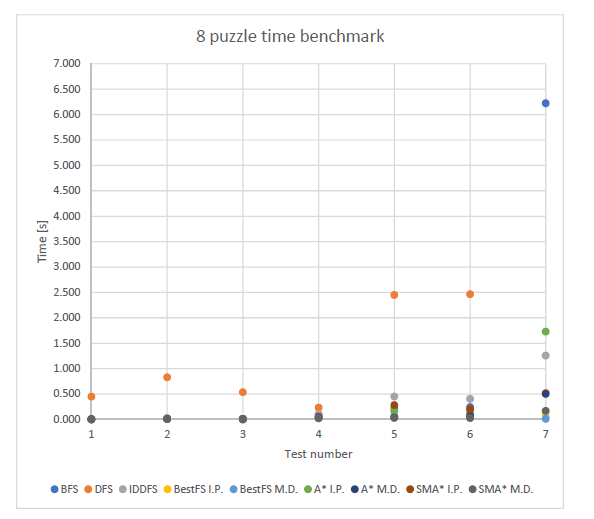
\includegraphics[width=0.75\textwidth]{8_puzzle_plot_basic}
    \centering
    \caption{8-puzzle time benchmark test results}
\label {eight-puzzle-plot}
\end{figure}

From this figure it is clear that in all tests except from 7th,  DFS algorithm was the slowest. In the last test BFS was the worst choice and it did not perform much better on other tests. Due to large differences in time measurements for BFS/DFS and other algorithms it is hard to find the best algorithm based on the plot provided. That is why the second plot in figure~\ref{eight-puzzle-plot-limited} was created which does not include BFS and DFS results. From this plot it is clear that the best algorithm cannot be stated, as it all depends on the type difficulty and configuration of a puzzle to be solved. Though in most cases IDDFS turned out to have the poorest performance. Surprisingly for last test A* with Incorrect Position heuristics turned out to be much worse than other algorithms. Depending on the test either Best First Search, A* or SMA* gave the best results. It can be stated that informed strategies performed much better than uninformed ones for the presented test cases.

 \begin{figure}[h]
    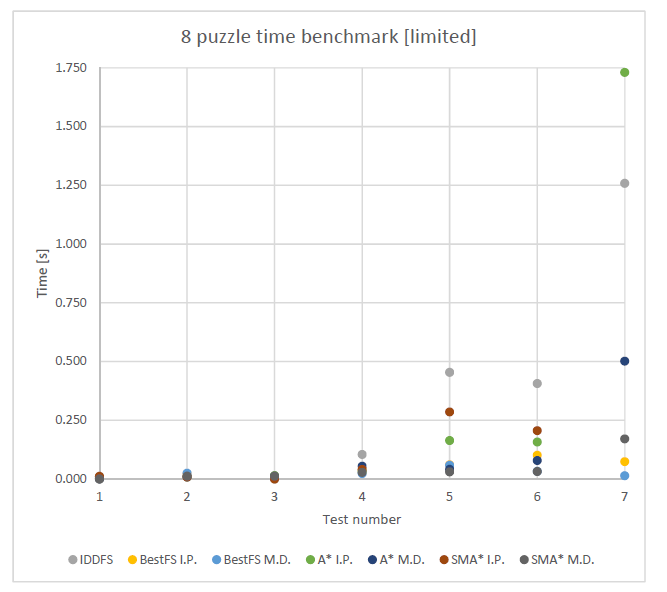
\includegraphics[width=0.75\textwidth]{8_puzzle_plot_limited}
    \centering
    \caption{8-puzzle time benchmark test results without BFS and DFS}
\label {eight-puzzle-plot-limited}
\end{figure}

Furthermore, a length of the solution is also a good predeterminant of an ability of a method to find optimal solutions. Figure ~\ref{eight-puzzle-plot-length} depicts what was the solution length for each test case.

 \begin{figure}[h]
    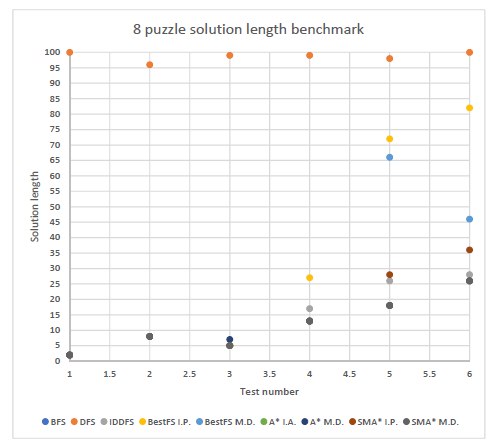
\includegraphics[width=0.75\textwidth]{8_puzzle_length}
    \centering
    \caption{8-puzzle solution length benchmark test results}
\label {eight-puzzle-plot-length}
\end{figure}

Due to the nature of DFS it always finds the solution that is has the largest length from all algorithms roughly equal to the depth limit of 100. For simple test cases, like test case 1, 2 and 3 there is almost no difference in solution length of all other algorithms. Only when test configuration are more complicated, differences in solution length start to be noticeable. For those test cases Best First Search with Incorrect Position Heuristics gave the worst results. Next there was Best First Search with Manhattan distance. Hence, we can judge that though being able to find the solution quickly, Best First Search algorithm does not find the most optimal solution. In all test cases, A* with both Incorrect Position heuristics and Manhattan Distance heuristics arrived with a solution of shortest path. Also SMA* with Manhattan Distance gave the same length of solution, while SMA* with the second type of heuristics required slightly more steps to achieve correct configuration. 

\newpage
\subsubsection {15-puzzle}

Similarly, for the 15-puzzle problem tile configurations from test cases were tested and their results gathered in the form of a table. This time, however, not only all algorithms with test 0 Heuristics were unable to solve the puzzle in acceptable time but also a DFS algorithm. That is why they will not be presented in a table of results~\ref{fifteen-puzzle-table}. 


\begin{longtable}[h]{|
>{\columncolor[HTML]{C0C0C0}}c ccccccccc|}
\caption{15-puzzle test results}
\label{fifteen-puzzle-table}\\
\hline
Method & \cellcolor[HTML]{C0C0C0} & \cellcolor[HTML]{C0C0C0} & \multicolumn{2}{c}{\cellcolor[HTML]{C0C0C0}BestFS} & \multicolumn{2}{c}{\cellcolor[HTML]{C0C0C0}A*} & \multicolumn{2}{c|}{\cellcolor[HTML]{C0C0C0}SMA*} \\
Heuristics & \multirow{-2}{*}{\cellcolor[HTML]{C0C0C0}BFS} & \multirow{-2}{*}{\cellcolor[HTML]{C0C0C0}IDFS} & \cellcolor[HTML]{C0C0C0}I.P. & \cellcolor[HTML]{C0C0C0}M.D. & \cellcolor[HTML]{C0C0C0}I.P. & \cellcolor[HTML]{C0C0C0}M.D. & \cellcolor[HTML]{C0C0C0}I.P. & \cellcolor[HTML]{C0C0C0}M.D. \\ \hline
\endfirsthead
%
\endhead
%
\hline
\endfoot
%
\endlastfoot
%
\multicolumn{9}{|c|}{\cellcolor[HTML]{EFEFEF}TEST 1} \\ \hline
Length & 3 & 3 & 3 & 3 & 3 & 3 & 3 & 3 \\
Iterations & 19 & 3 & 4 & 5 & 4 & 5 & 13 & 14 \\
Time & 0.010 & 0.01 & 0.01 & 0.024 & 0.010 & 0.016 & 0.011 & 0.009 \\ \hline
\multicolumn{9}{|c|}{\cellcolor[HTML]{EFEFEF}TEST 2} \\ \hline
Length & 5 & 5 & 5 & 5 & 5 & 5 & 5 & 5 \\
Iterations & 83 & 5 & 6 & 7 & 6 & 7 & 18 & 18 \\
Time & 0.008 & 0.008 & 0.013 & 0.002 & 0.003 & 0.007 & 0.007 & 0.003 \\ \hline
\multicolumn{9}{|c|}{\cellcolor[HTML]{EFEFEF}TEST 3} \\ \hline
Length & 14 & 24 & 156 & 168 & 14 & 14 & 14 & 14 \\
Iterations & 78520 & 24 & 7287 & 11026 & 82 & 83 & 293 & 265 \\
Time & 1.666 & 16.672 & 0.571 & 1.056 & 0.005 & 0.018 & 0.005 & 0.010 \\ \hline
\multicolumn{9}{|c|}{\cellcolor[HTML]{EFEFEF}TEST 4} \\ \hline
Length & 16 & 16 & 50 & 20 & 16 & 16 & 16 & 16 \\
Iterations & 413213 & 16 & 1234 & 176 & 203 & 125 & 472 & 444 \\
Time & 27.856 & 1.219 & 0.146 & 0.03 & 0.018 & 0.017 & 0.031 & 0.021 \\ \hline
\multicolumn{9}{|c|}{\cellcolor[HTML]{EFEFEF}TEST 5} \\ \hline
Length & 16 & 20 & 114 & 50 & 16 & 16 & 20 & 16 \\
Iterations & 369296 & 20 & 1645 & 148 & 992 & 503 & 28682 & 2624 \\
Time & 10.783 & 4.955 & 0.296 & 0.039 & 0.053 & 0.032 & 7.324 & 0.105 \\ \hline
\multicolumn{9}{|c|}{\cellcolor[HTML]{EFEFEF}TEST 6} \\ \hline
Length & - & - & 78 & 138 & 24 & 24 & 28 & 30 \\
Iterations & - & - & 913 & 16286 & 33782 & 4467 & 110953 & 76123 \\
Time & - & - & 0.049 & 1.096 & 2.343 & 0.329 & 178.558 & 68.247 \\ \hline
\end{longtable}
 
As in case of 8-puzzle, for 15-puzzle a plot of time needed for all algorithms to complete is presented in figure ~\ref{fifteen-puzzle-plot}.

\begin{figure}[h]
    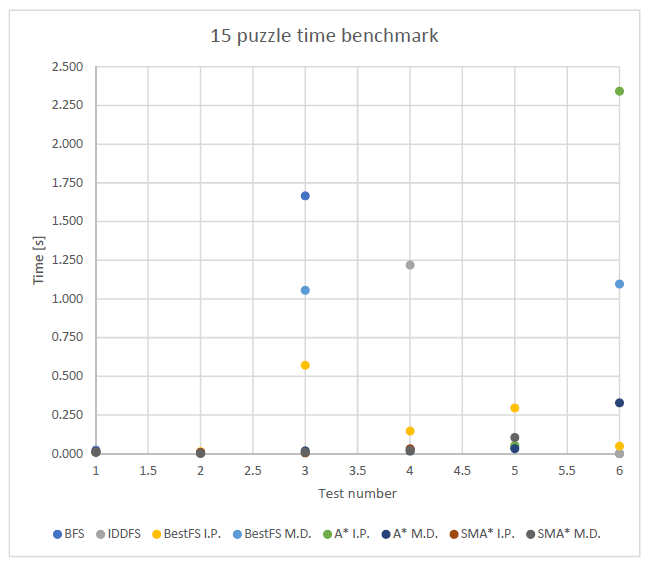
\includegraphics[width=0.75\textwidth]{15_puzzle_plot}
    \centering
    \caption{15-puzzle time benchmark test results}
\label {fifteen-puzzle-plot}
\end{figure}

In this plot largest numbers were omitted, as they exceed largely the average time spend on each test. For the last test the worst method which is SMA* with Incorrect Position Heuristics was over 3500 times slower than the best method - Best First Search with Incorrect Position Heuristics. Not to mention that BFS, and IDDFS took to long to even measure their efficiency. Once again, depending on the test sample, either Best First Search, A* or SMA* gave the best results and in the first test samples they were quite similar. Only after 4th sample SMA* drastically deteriorated in performance.    

Next analysis of performance will be devoted to length of the solution found. Plot representing it is shown if figure  ~\ref{fifteen-puzzle-plot-length}.

 \begin{figure}[h]
    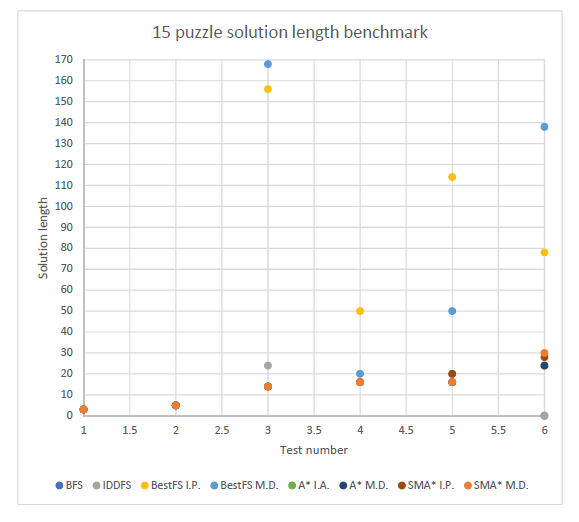
\includegraphics[width=0.75\textwidth]{15_puzzle_length}
    \centering
    \caption{15-puzzle solution length benchmark test results}
\label {fifteen-puzzle-plot-length}
\end{figure}

Once again A* algorithm was the one to always arrive with the shortest path to the solution. Until 4th test also SMA* was able to find a solution with the same length. In test 5 and 6, even tough it took an awful lot of time still the final result was close to optimal. Best First Search algorithm was the one to find solutions of longest paths.

\section {Conclusions}

In this project, six different algorithms were implemented, in order to solve an 8 and 15-puzzle problem. Three of those algorithms, namely BFS, DFS and IDDFS were uninformed algorithms, while BestFS, A* and SMA* were informed algorithms. For the latter group, two types of heuristics were implemented: Incorrect Position and Manhattan Distance. All algorithms were tested with 12 test cases, 6 per each puzzle type.

All test were performed on local environment which was not closed, hence, some other processes of the operating system may have influenced the results. However, even with such a small number of test cases and limits of the test environment, the behaviour of algorithms could be observed. In general, informed algorithms  performed much better than uninformed algorithms, both when it comes to processing time and length of a solution. For difficult and large puzzles, SMA* took a lot more time than other informed algorithms, however, it arrived with an almost optimal solution. In many test cases, Best First Search required the least amount of time, however, the path found was sometimes much longer than the path found by other algorithms. On the other hand, A* in all test cases resulted in the shortest possible path that was found with the shortest  or close to the shortest execution time. DFS was the algorithm that performed very poorly, especially in 15-puzzle problem. BFS usually took more time, but it arrived at a solution in all test cases except the most complicated one. When it comes to the comparison of heuristics it is all dependent on the initial tile configuration. For some tests Incorrect Position Heuristics gave better results, while for the other Manhattan Distance. The importance of proper choice of heuristics was proved with use of test 0 heuristics, which was not able to solve even the simplest puzzles in time comparable to other algorithms. 

Depending on whether the time of execution is more important, or finding the shortest path, either Best First Search or A* should be used to tackle the problem of puzzle solving. 



\newpage
\listoffigures
\newpage
\printbibliography

\end{document}




